\subsection{External interfaces requirements}
\subsubsection{User interfaces}
\begin{enumerate}[label=\textbf{R\arabic*}]
    \item The \ac{eMSP} must allow the users to register (providing email, password, payment method and his infos);
    \item The \ac{CPMS} must allow the \acp{CPO} to register (providing email, password, id-station, partita iva, number of possible charging slots);
    \item The system must allow the \acp{CPO} to modify the possible charging slots in their stations;
          % Maybe not useful anymore R4
    \item The system must verify the correctness of the identification data for the \acp{CPO};
    \item The system must allow the user to login;
    \item The system must allow the user to choose a specific station, a timeslot;
    \item The system must notify the user when the charging process is finished via a notification;
    \item The \ac{CPMS} must allow the \acp{CPO} to choose the mode (manual or automatic) of operation
\end{enumerate}
\subsubsection{Hardware interfaces}
\subsubsection{Software interfaces}
\subsubsection{Communication interfaces}

\subsection{Functional requirements}

\begin{enumerate}[label=\textbf{R\arabic*}]
    \item The system must provide information () about the stations nearby;
    \item The system must reserve a position for a user who registered for a charge through the application;
    \item The system mustn't have collisions in the booking of charges; (non si possono registrare più di X user per timeslot sovrapposti)
    \item The system must take the service money from the user payment method after the charging is finished;
\end{enumerate}
\clearpage
\subsubsection{Sequence diagrams}
\todo[inline]{Per quanto riguarda il sistema CPMS, come si "registra" il CPO maintainer?}
Below there are some sequence diagrams to show how the basic actions should be over time.
\begin{figure}[!h]
    \begin{center}
        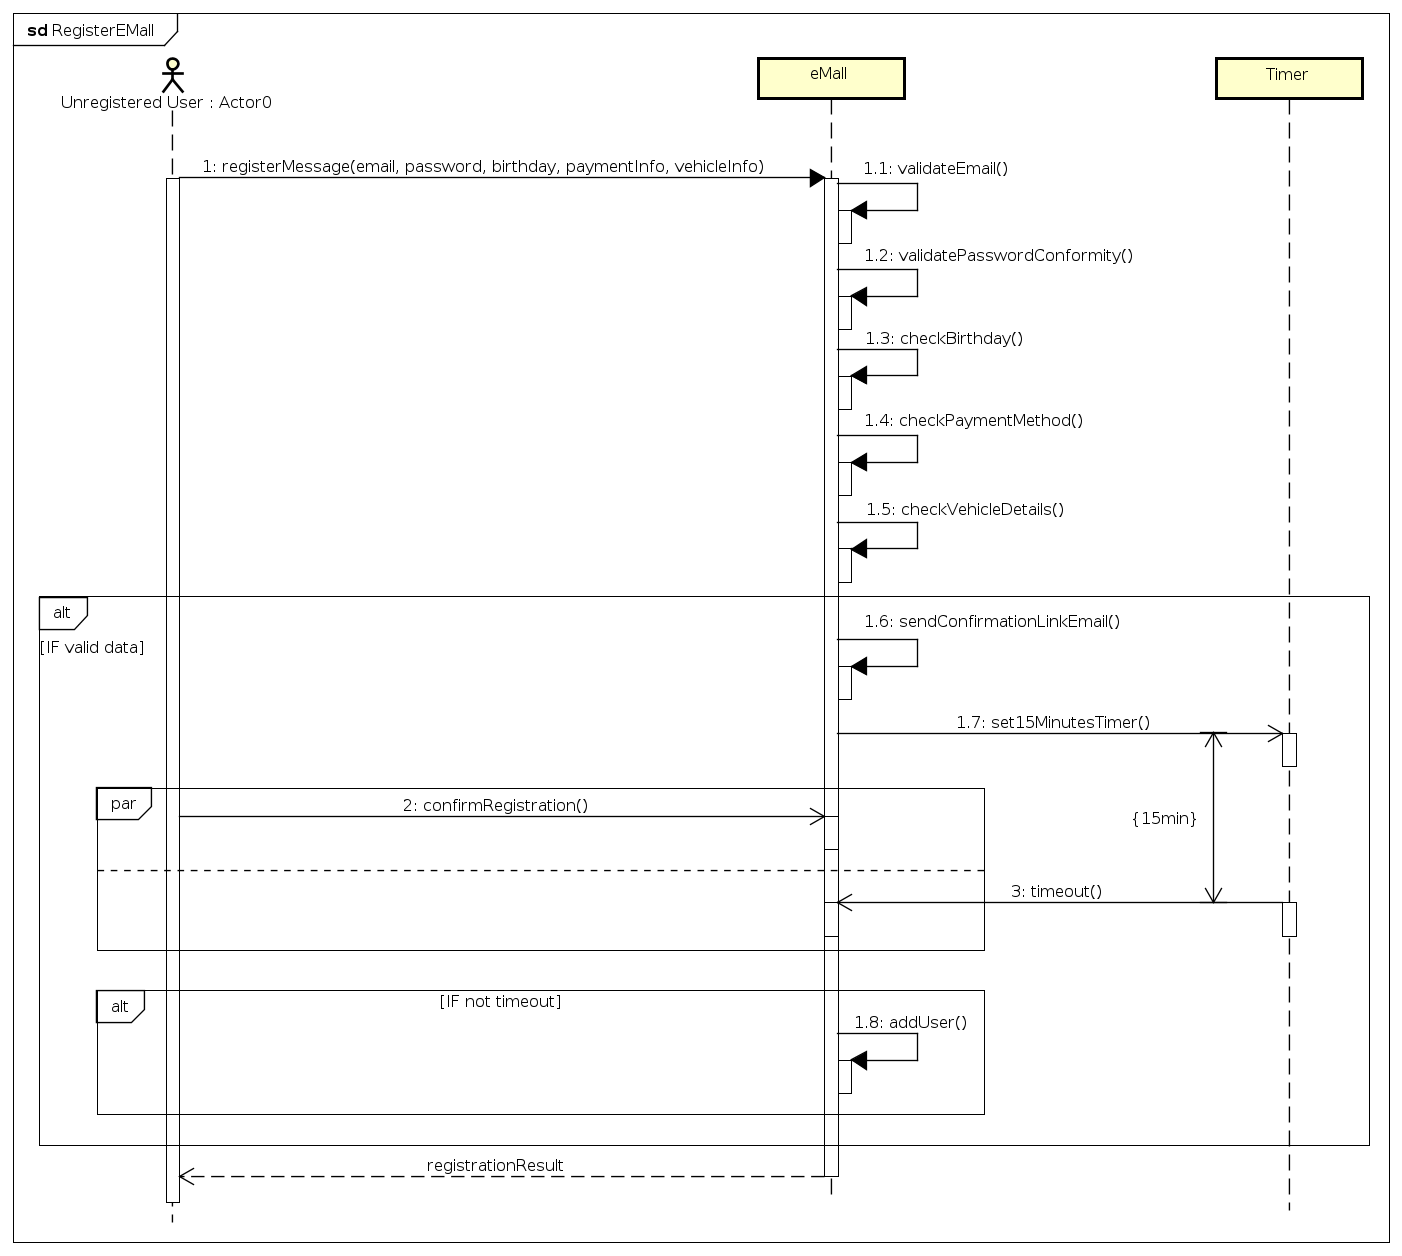
\includegraphics[keepaspectratio, width=16cm]{Sequence/RegisterEMall.png}
        \caption{Registration into \ac{eMall} sequence}
    \end{center}
\end{figure}
\begin{figure}[!h]
    \begin{center}
        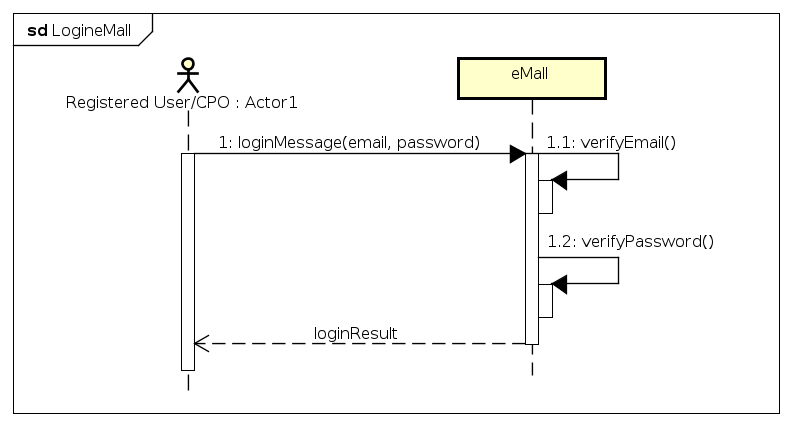
\includegraphics[keepaspectratio, width=16cm]{Sequence/LoginEMall.png}
        \caption{Login into \ac{eMall} sequence}
    \end{center}
\end{figure}
\begin{figure}[!h]
    \begin{center}
        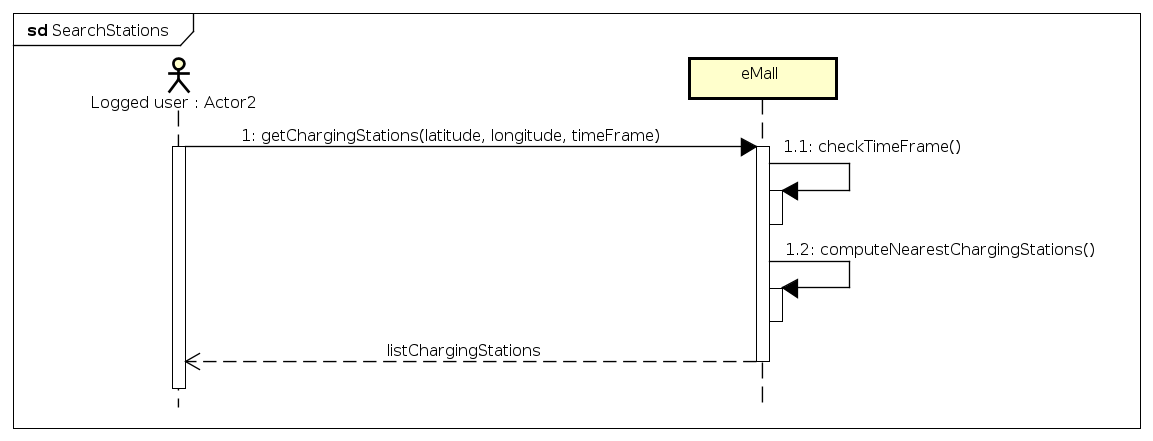
\includegraphics[keepaspectratio, width=16cm]{Sequence/SearchStations.png}
        \caption{Get the nearby charging stations}
    \end{center}
\end{figure}
\begin{figure}[!h]
    \begin{center}
        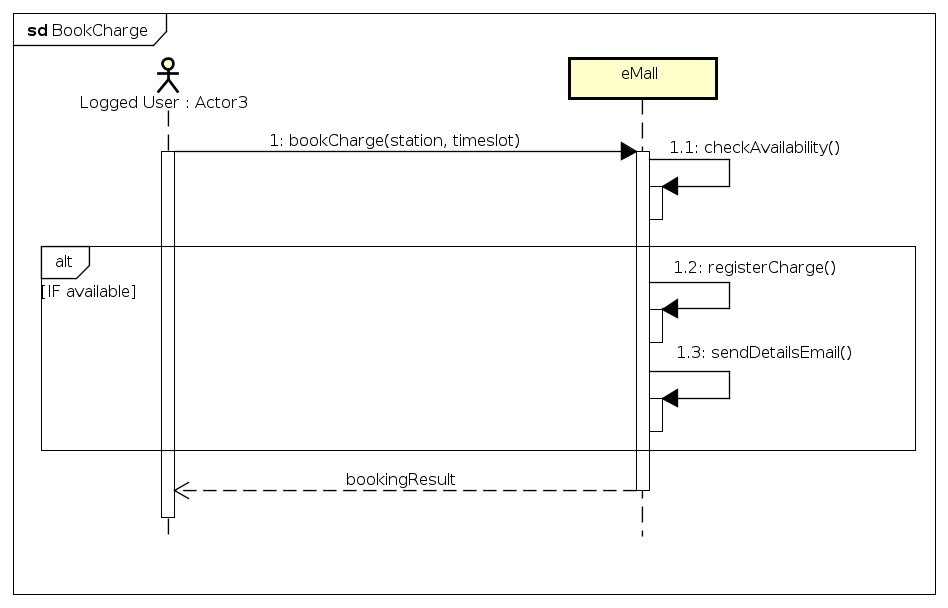
\includegraphics[keepaspectratio, width=16cm]{Sequence/BookCharge.png}
        \caption{Book a charge sequence}
    \end{center}
\end{figure}
\begin{figure}[!h]
    \begin{center}
        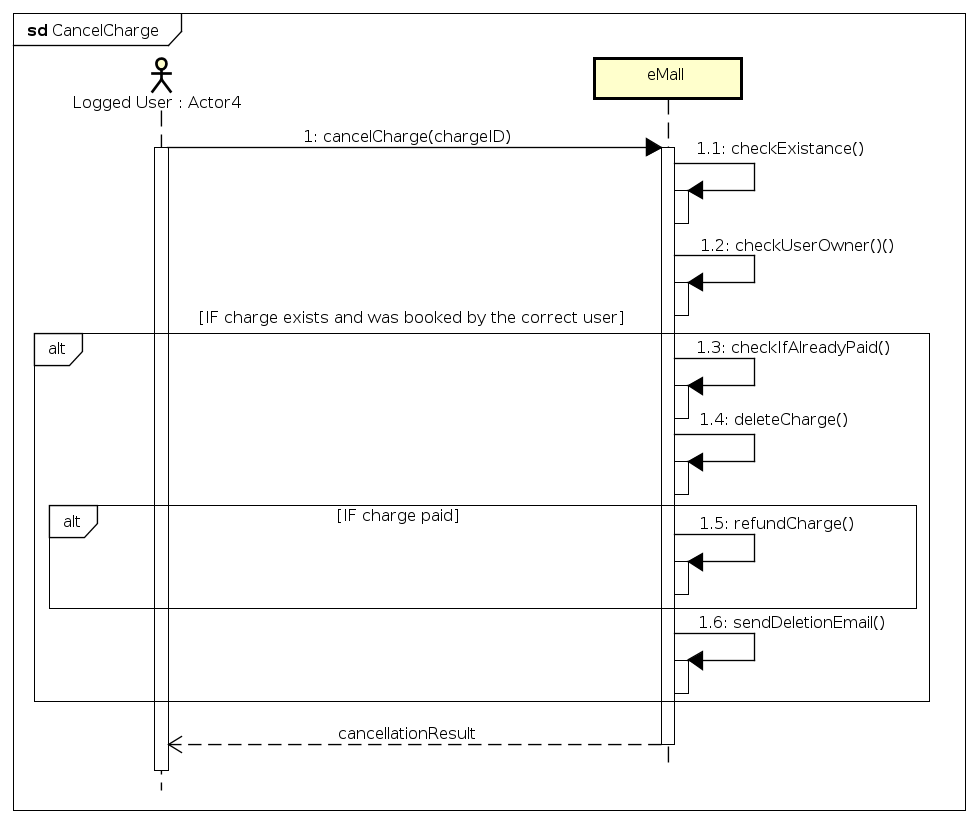
\includegraphics[keepaspectratio, width=16cm]{Sequence/CancelCharge.png}
        \caption{Cancel a charge sequence}
    \end{center}
\end{figure}
\clearpage
%Definition of use case diagrams, use cases and associated sequence/activity diagrams, and mapping on requirements
\subsection{Performance requirements}

\subsection{Design constraints}
\subsubsection{Standards compliance}
\subsubsection{Hardware limitations}
\subsubsection{Other constraints (TODO MAYBE)}

\subsection{Software system attributes}
\subsubsection{Reliability}
\subsubsection{Availability}
\subsubsection{Security}
\subsubsection{Maintainability}
\subsubsection{Portability}
\subsection{Requirements}
\subsubsection{External Interface Requirements}
\clearpage